

\begin{itemize}
 \item Informacion sobre la cantidad de unidades involucradas en las transacciones.
\begin{kframe}
\begin{alltt}
 \hlstd{summarizeQuantity} \hlkwb{=} \hlkwd{data.frame}\hlstd{(}\hlkwc{cantidad} \hlstd{= onlineRetails}\hlopt{$}\hlstd{Quantity);}
 \hlkwd{stargazer}\hlstd{(summarizeQuantity);}
\end{alltt}
\end{kframe}
% Table created by stargazer v.5.2 by Marek Hlavac, Harvard University. E-mail: hlavac at fas.harvard.edu
% Date and time: sáb, abr 09, 2016 - 09:48:52
\begin{table}[!htbp] \centering 
  \caption{} 
  \label{} 
\begin{tabular}{@{\extracolsep{5pt}}lccccc} 
\\[-1.8ex]\hline 
\hline \\[-1.8ex] 
Statistic & \multicolumn{1}{c}{N} & \multicolumn{1}{c}{Mean} & \multicolumn{1}{c}{St. Dev.} & \multicolumn{1}{c}{Min} & \multicolumn{1}{c}{Max} \\ 
\hline \\[-1.8ex] 
cantidad & 541,909 & 9.552 & 218.081 & $-$80,995 & 80,995 \\ 
\hline \\[-1.8ex] 
\end{tabular} 
\end{table} 

 \item Información correspondiente al periodo de tiempo de la medicion.
 
 \begin{itemize}
  \item Fecha inicial 
\begin{kframe}
\begin{alltt}
 \hlkwd{print}\hlstd{(range[}\hlnum{1}\hlstd{])}
\end{alltt}
\end{kframe}[1] "2010-01-12"

  \item Fecha Final 
\begin{knitrout}
\definecolor{shadecolor}{rgb}{0.969, 0.969, 0.969}\color{fgcolor}\begin{kframe}
\begin{alltt}
 \hlkwd{print}\hlstd{(range[}\hlnum{2}\hlstd{])}
\end{alltt}
\begin{verbatim}
## [1] "2011-12-10"
\end{verbatim}
\end{kframe}
\end{knitrout}
 \end{itemize} 
  
 \item Información correspondiente a los productos.
\begin{knitrout}
\definecolor{shadecolor}{rgb}{0.969, 0.969, 0.969}\color{fgcolor}\begin{kframe}
\begin{alltt}
 \hlstd{summarizeUnitPrice} \hlkwb{=} \hlkwd{data.frame}\hlstd{(}\hlkwc{precioUnitario} \hlstd{= onlineRetails}\hlopt{$}\hlstd{UnitPrice);}
 \hlkwd{stargazer}\hlstd{(summarizeUnitPrice);}
\end{alltt}
\begin{verbatim}
## 
## % Table created by stargazer v.5.2 by Marek Hlavac, Harvard University. E-mail: hlavac at fas.harvard.edu
## % Date and time: sáb, abr 09, 2016 - 09:48:53
## \begin{table}[!htbp] \centering 
##   \caption{} 
##   \label{} 
## \begin{tabular}{@{\extracolsep{5pt}}lccccc} 
## \\[-1.8ex]\hline 
## \hline \\[-1.8ex] 
## Statistic & \multicolumn{1}{c}{N} & \multicolumn{1}{c}{Mean} & \multicolumn{1}{c}{St. Dev.} & \multicolumn{1}{c}{Min} & \multicolumn{1}{c}{Max} \\ 
## \hline \\[-1.8ex] 
## precioUnitario & 541,909 & 4.611 & 96.760 & $-$11,062.060 & 38,970.000 \\ 
## \hline \\[-1.8ex] 
## \end{tabular} 
## \end{table}
\end{verbatim}
\end{kframe}
\end{knitrout}
 
 \item Para conocer el producto mas vendido, se procede con una grafica que contiene la cantidad de productos por unidad vendidos
\begin{knitrout}
\definecolor{shadecolor}{rgb}{0.969, 0.969, 0.969}\color{fgcolor}\begin{kframe}
\begin{alltt}
\hlkwd{ggplot}\hlstd{(onlineRetails,}\hlkwd{aes}\hlstd{(}\hlkwc{x}\hlstd{=StockCode,} \hlkwc{y} \hlstd{= Quantity))} \hlopt{+} \hlkwd{geom_bar}\hlstd{(}\hlkwc{stat}\hlstd{=}\hlstr{"identity"}\hlstd{)} \hlopt{+} \hlkwd{theme}\hlstd{(}\hlkwc{axis.text.x}\hlstd{=}\hlkwd{element_blank}\hlstd{())}
\end{alltt}


{\ttfamily\noindent\color{warningcolor}{\#\# Warning: Stacking not well defined when ymin != 0}}\end{kframe}
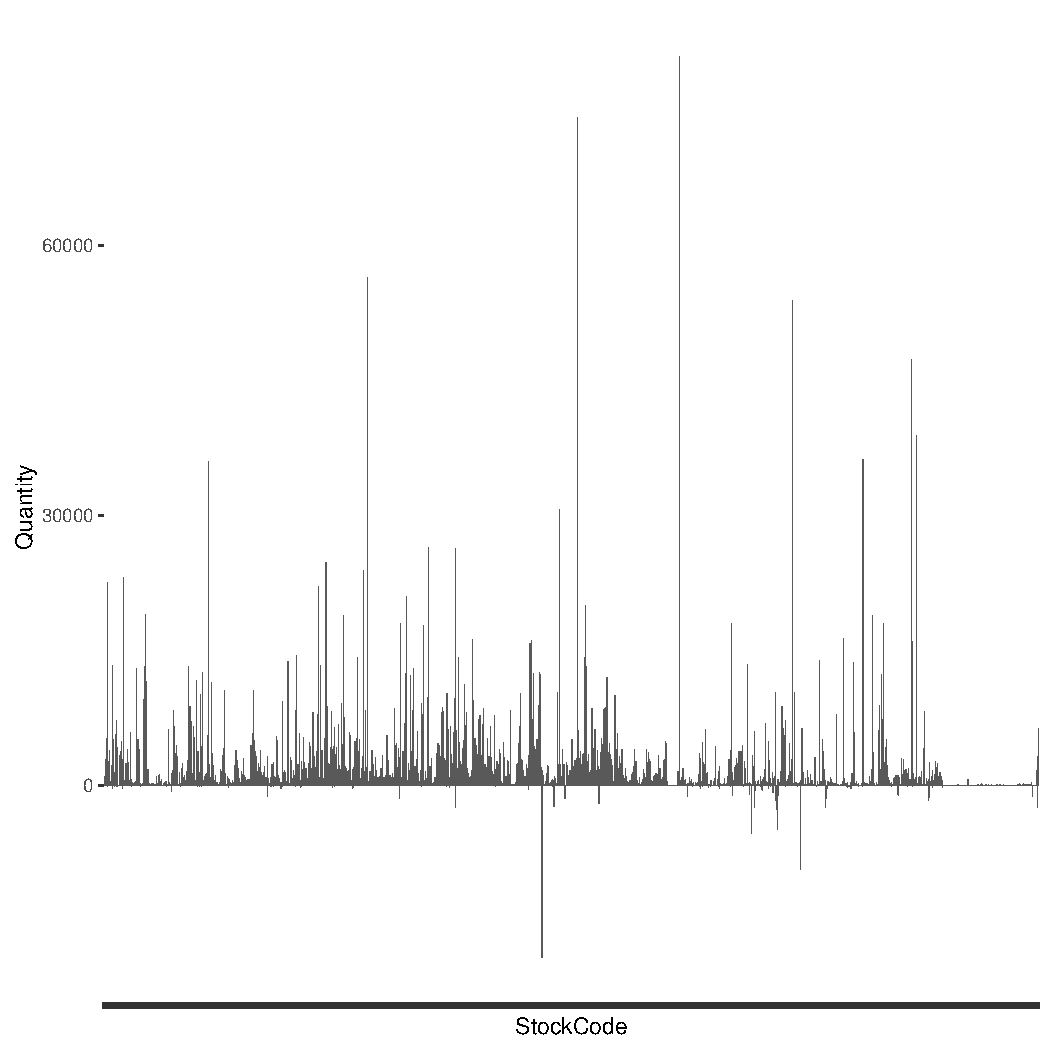
\includegraphics[width=\maxwidth]{figure/grafico_productos-1} 

\end{knitrout}

  \item Para conocer los registros de ventas de las transacciones se grafica la informacion de las transacciones diarias.
\begin{knitrout}
\definecolor{shadecolor}{rgb}{0.969, 0.969, 0.969}\color{fgcolor}\begin{kframe}
\begin{alltt}
\hlkwd{ggplot}\hlstd{(onlineRetails,}\hlkwd{aes}\hlstd{(}\hlkwc{x}\hlstd{=Date,} \hlkwc{y} \hlstd{= Quantity}\hlopt{*}\hlstd{UnitPrice))} \hlopt{+} \hlkwd{geom_bar}\hlstd{(}\hlkwc{stat}\hlstd{=}\hlstr{"identity"}\hlstd{)}
\end{alltt}


{\ttfamily\noindent\color{warningcolor}{\#\# Warning: Removed 308950 rows containing missing values (position\_stack).}}

{\ttfamily\noindent\color{warningcolor}{\#\# Warning: Stacking not well defined when ymin != 0}}\end{kframe}
\includegraphics[width=\maxwidth]{figure/histograma_transacciones-1} 

\end{knitrout}
  
\end{itemize}




